\chapter{Mobilidade em São Paulo}
\label{cap:mobilidade-rmsp}

Para fornecer uma melhor compreensão do cenário de nossa análise, esta seção
descreve as características da Região Metropolitana de S\~ao Paulo e os dados da
última pesquisa OD realizada na região. Para evitar antagonismos entre a
Região Metropolitana de S\~ao Paulo Área (RMSP) e a cidade de S\~ao Paulo, vamos nos
referir à cidade como capital ou simplesmente S\~ao Paulo e vamos nos referir à
área metropolitana como RMSP ou simplesmente área metropolitana. 

\section{Região Metropolitana de São Paulo}

O estado de S\~ao Paulo está localizado no litoral sudeste do Brasil. A Regi\~ao
Metropolitana de S\~ao Paulo é a região mais populosa da América do Sul. De acordo
com o Instituto Brasileiro de Geografia e Estatística \citep{ibge2020}, a RMSP contabilizou $21,9$
milhões de cidadãos em 2020, o que representa cerca de 10\% da população
brasileira. A RMSP é composta por 39 municípios em uma área de \num{7946.84} $km^{2}$. A
cidade de São Paulo é a capital do estado de São Paulo e está localizada no
centro da região metropolitana. A Figura \ref{fig:map-spma} mostra os 39 municípios que compõem a
RMSP. A capital é a cidade mais populosa do Brasil, com 12.3 milhões de
habitantes. Na RMSP, as outras cidades com mais habitantes são Guarulhos (1.4
milhão), São Bernardo do Campo (844 mil), Santo André (721 mil) e Osasco (699
mil).

\begin{figure}[!htb]
  \centering
  \captionsetup{justification=centering}
  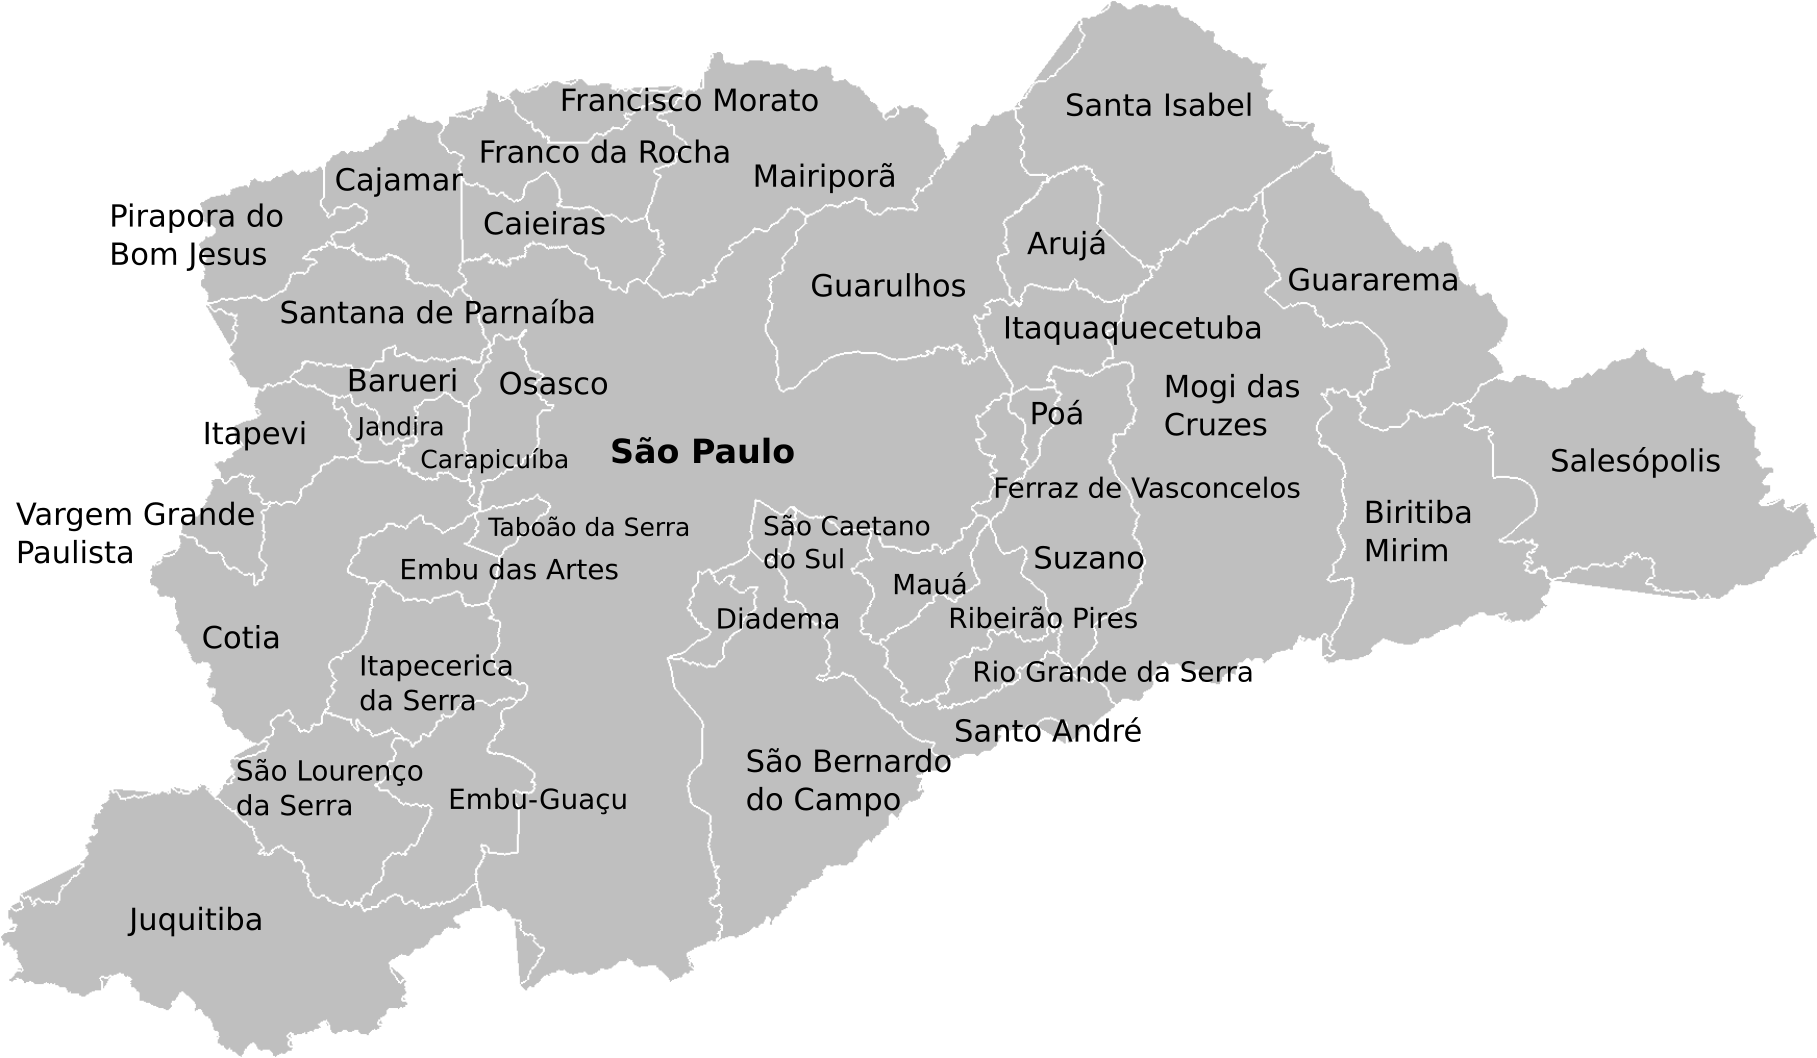
\includegraphics[width=0.95\textwidth]{../figuras/map-spma.png}
    \caption{Municípios da RMSP.\label{fig:map-spma}}
\end{figure}

A capital e as cidades mais próximas concentram a maior parte das oportunidades
de emprego, instalações e serviços públicos, universidades, museus e opções
de entretenimento. Portanto, há um grande deslocamento diário para o centro da
capital e seus arredores. Em São Paulo, os bairros próximos ao centro da
cidade são mais valorizados, portanto, morar nessas partes da cidade tem um maior custo.
Pessoas com menos condições financeiras costumam residir na periferia da capital
ou em outras cidades da RMSP, por isso, algumas cidades da RMSP tornaram-se cidades
dormitório para aqueles que não podem pagar comprar ou alugar uma casa na
capital.

Em relação à infraestrutura de transporte, a capital possui uma rede metroviária
que atende as regiões norte, sul, leste, oeste, sudoeste e sudeste da cidade.
Existem algumas linhas de metrô, a maioria delas cruzando o centro da capital, o
que limita o acesso ao sistema de metrô a algumas regiões da cidade. As demais
cidades não possuem sistemas de metrô, mas existe um outro sistema ferroviário
metropolitano que atende várias cidades do entorno e que é integrado ao sistema
metroviário da capital.

Cada cidade tem seu próprio sistema de ônibus e há um sistema de ônibus
intermunicipal para ligar o cidades vizinhas. Durante o século 20 até o final da
década de 1990, a maioria dos investimentos no transporte foram guiados por uma
abordagem focada no transporte individual de carros em detrimento do transporte
público \cite{rolnik2011}. Os objetivos eram ampliar estradas e ruas para
atender à crescente demanda por carros particulares. Nas últimas duas décadas,
os governos locais têm investido mais em políticas de incentivo ao transporte
público, como implantação de corredores de ônibus e substituição da frota de
ônibus, construção de novas linhas de metrô e modernização do sistema
ferroviário. Além disso, há uma crescente infraestrutura de ciclismo na capital
que vem sendo expandida na última década. Embora esses investimentos tenham
aumentado nos últimos anos, a RMSP ainda sofre com o congestionamento do
tráfego, principalmente nos horários de pico \cite{rolnik2011,ricardo:18}.
Assim, é necessário um melhor entendimento do o comportamento do trânsito na
RMSP para propor novas políticas de melhoria da mobilidade para seus cidadãos.

\section{Pesquisa Origem-Destino}
